% autosearch_figures.tex — TikZ figures for the autonomous feature selection protocol
% Compile with: pdflatex autosearch_figures.tex (x2 for pgfplots)
\documentclass[border=10pt]{standalone}
\usepackage[utf8]{inputenc}
\usepackage{tikz}
\usepackage{pgfplots}
\usepackage{algorithm2e}
\usepackage{amsmath,amssymb}
\usepackage{xcolor}

\usetikzlibrary{
  shapes.geometric,
  arrows.meta,
  positioning,
  fit,
  backgrounds,
  calc,
  decorations.pathreplacing
}
\pgfplotsset{compat=1.18}

% Colour palette
\definecolor{keepgreen}{HTML}{2E8B57}
\definecolor{discardred}{HTML}{CD3333}
\definecolor{crashorange}{HTML}{FF8C00}
\definecolor{llmpurple}{HTML}{7B68EE}
\definecolor{trainblue}{HTML}{4682B4}
\definecolor{gitgray}{HTML}{555555}
\definecolor{bglight}{HTML}{F5F5F5}
\definecolor{phasebg}{HTML}{E8E8F0}
\definecolor{bugred}{HTML}{FF4444}

\begin{document}

% ================================================================
% FIGURE 1 — Protocol Diagram (Flowchart)
% ================================================================
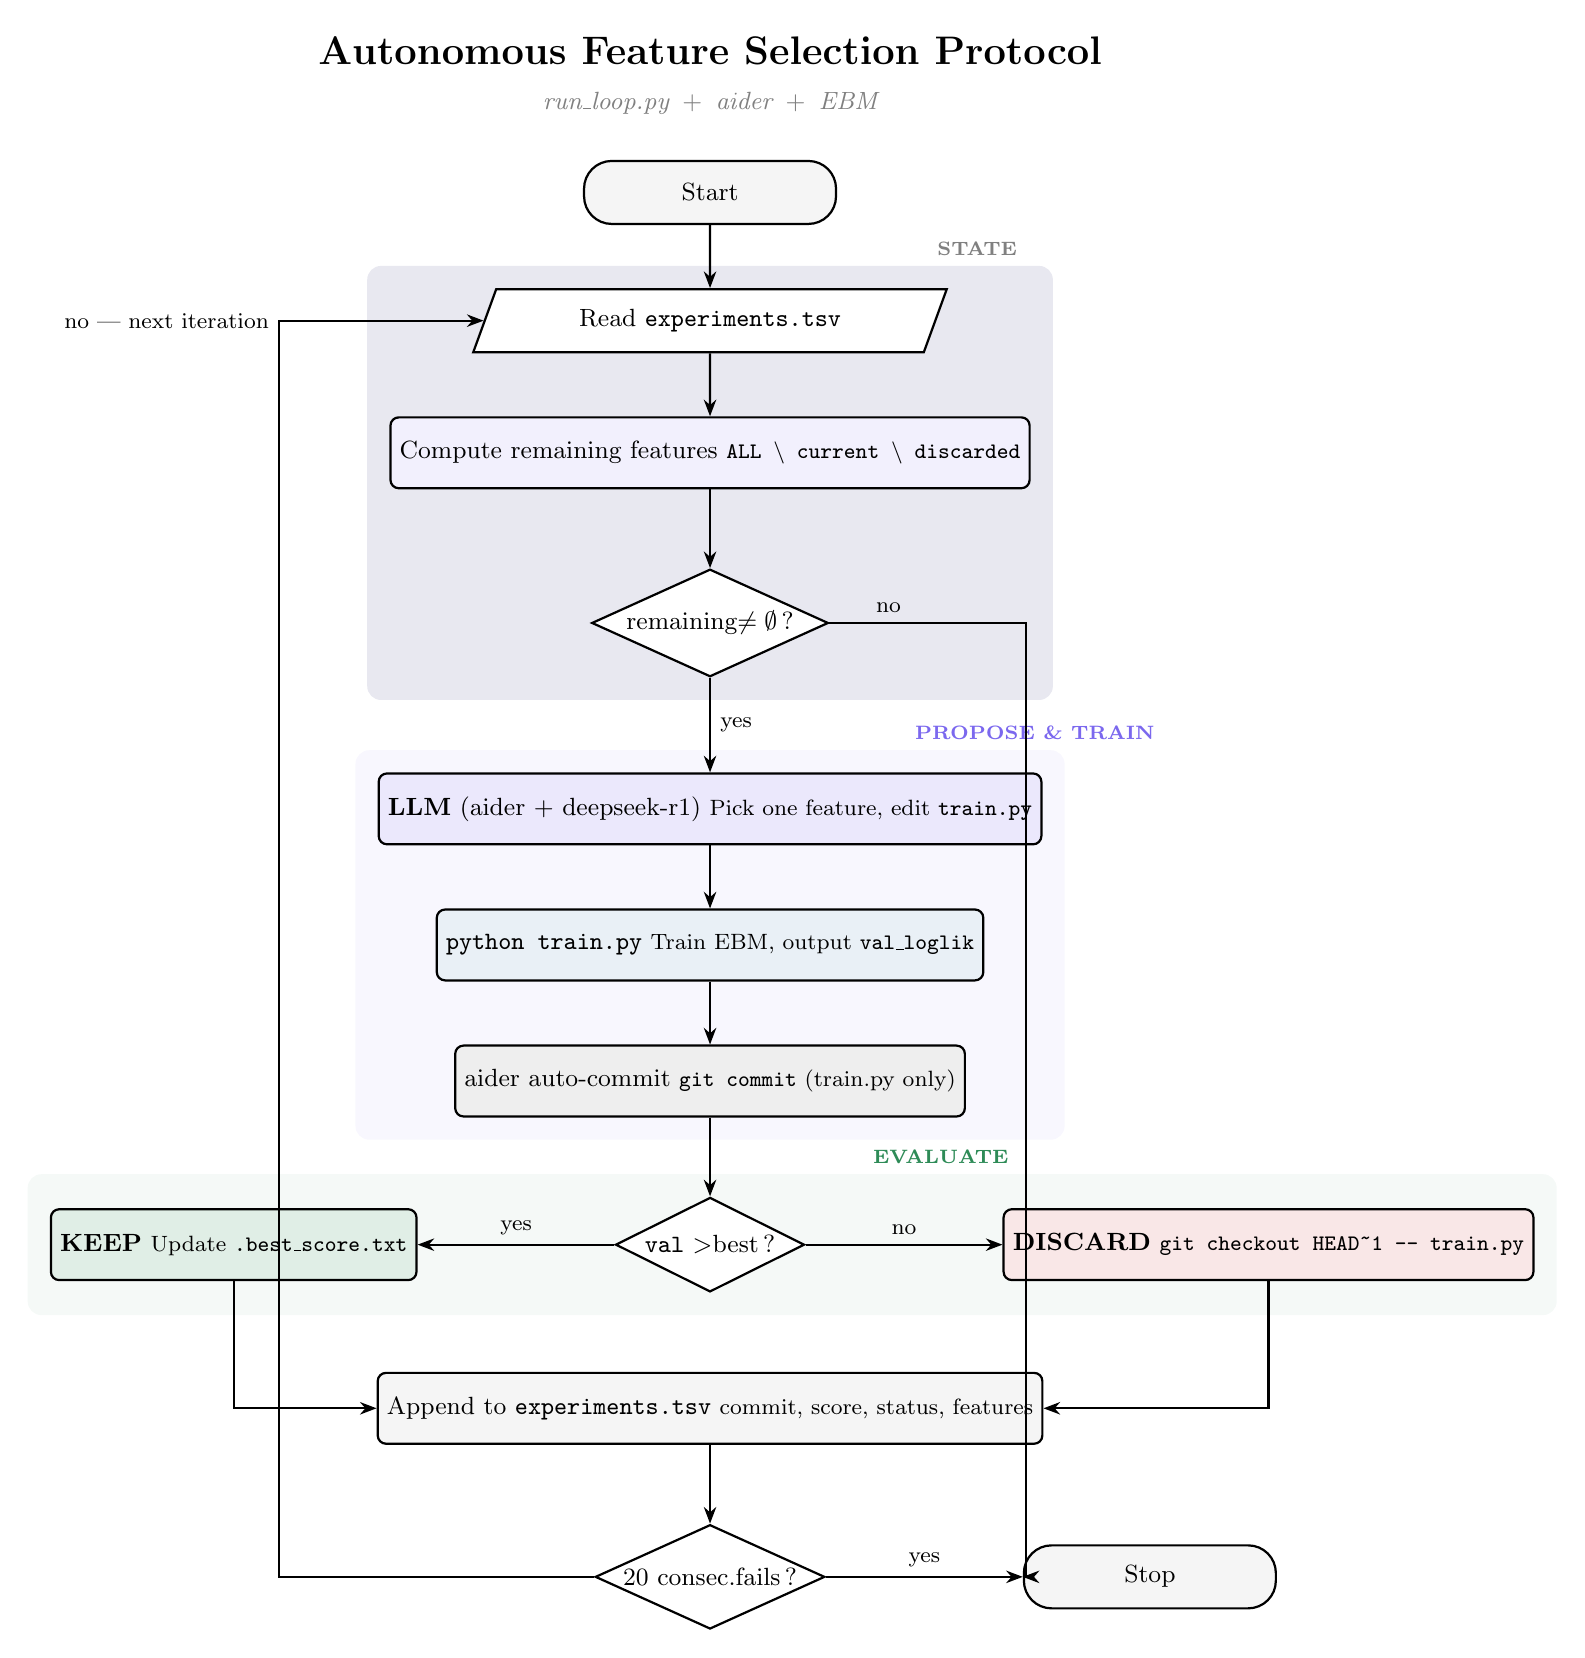
\begin{tikzpicture}[
    node distance=1.2cm and 2.5cm,
    every node/.style={font=\small},
    process/.style={
      rectangle, draw, rounded corners=3pt,
      minimum width=3.8cm, minimum height=0.9cm,
      fill=white, thick
    },
    decision/.style={
      diamond, draw, thick,
      minimum width=2.2cm, minimum height=1.2cm,
      inner sep=1pt, fill=white,
      aspect=2.2
    },
    startstop/.style={
      rectangle, draw, rounded corners=10pt,
      minimum width=3.2cm, minimum height=0.8cm,
      fill=bglight, thick
    },
    io/.style={
      trapezium, draw, thick,
      trapezium left angle=70, trapezium right angle=110,
      minimum width=3cm, minimum height=0.8cm,
      fill=white
    },
    arrow/.style={-{Stealth[length=6pt]}, thick},
    dasharrow/.style={-{Stealth[length=5pt]}, thick, dashed, gray},
  ]

  % --- Title ---
  \node[font=\Large\bfseries, anchor=south] at (0, 11.5)
    {Autonomous Feature Selection Protocol};
  \node[font=\small\itshape, anchor=north, text=gray] at (0, 11.4)
    {run\_loop.py $\,+\,$ aider $\,+\,$ EBM};

  % --- Nodes ---
  \node[startstop] (start) at (0, 10) {Start};

  \node[io, below=0.8cm of start] (readstate)
    {Read \texttt{experiments.tsv}};

  \node[process, below=0.8cm of readstate, fill=llmpurple!10] (remaining)
    {Compute remaining features\\[-2pt]
     {\footnotesize\texttt{ALL $\setminus$ current $\setminus$ discarded}}};

  \node[decision, below=1cm of remaining] (anyleft)
    {remaining\\$\neq \emptyset$\,?};

  \node[process, below=1.2cm of anyleft, fill=llmpurple!15] (llm)
    {\textbf{LLM} (aider + deepseek-r1)\\[-2pt]
     {\footnotesize Pick one feature, edit \texttt{train.py}}};

  \node[process, below=0.8cm of llm, fill=trainblue!12] (train)
    {\texttt{python train.py}\\[-2pt]
     {\footnotesize Train EBM, output \texttt{val\_loglik}}};

  \node[process, below=0.8cm of train, fill=gitgray!10] (commit)
    {aider auto-commit\\[-2pt]
     {\footnotesize \texttt{git commit} (train.py only)}};

  \node[decision, below=1cm of commit] (improved)
    {\texttt{val} $>$\\best\,?};

  % Keep branch (left)
  \node[process, left=2.5cm of improved, fill=keepgreen!15] (keep)
    {\textbf{KEEP}\\[-2pt]
     {\footnotesize Update \texttt{.best\_score.txt}}};

  % Discard branch (right)
  \node[process, right=2.5cm of improved, fill=discardred!12] (discard)
    {\textbf{DISCARD}\\[-2pt]
     {\footnotesize \texttt{git checkout HEAD\textasciitilde1 -- train.py}}};

  \node[process, below=1cm of improved, fill=bglight] (log)
    {Append to \texttt{experiments.tsv}\\[-2pt]
     {\footnotesize commit, score, status, features}};

  \node[decision, below=1cm of log] (stopcheck)
    {20 consec.\\fails\,?};

  \node[startstop, right=2.5cm of stopcheck] (stop) {Stop};

  % --- Arrows ---
  \draw[arrow] (start) -- (readstate);
  \draw[arrow] (readstate) -- (remaining);
  \draw[arrow] (remaining) -- (anyleft);

  \draw[arrow] (anyleft) -- node[right, font=\footnotesize] {yes} (llm);
  \draw[arrow] (anyleft.east) -- ++(2.5,0) node[above, font=\footnotesize, pos=0.3] {no}
    |- (stop);

  \draw[arrow] (llm) -- (train);
  \draw[arrow] (train) -- (commit);
  \draw[arrow] (commit) -- (improved);

  \draw[arrow] (improved.west) -- node[above, font=\footnotesize] {yes} (keep);
  \draw[arrow] (improved.east) -- node[above, font=\footnotesize] {no} (discard);

  \draw[arrow] (keep.south) |- (log);
  \draw[arrow] (discard.south) |- (log);

  \draw[arrow] (log) -- (stopcheck);
  \draw[arrow] (stopcheck.east) -- node[above, font=\footnotesize] {yes} (stop);
  \draw[arrow] (stopcheck.west) -| ([xshift=-4cm]stopcheck.west)
    |- (readstate.west)
    node[left, font=\footnotesize, pos=0.5] {no — next iteration};

  % --- Phase labels (right side) ---
  \begin{scope}[on background layer]
    \node[fit=(readstate)(remaining)(anyleft),
      fill=phasebg, rounded corners=5pt, inner sep=8pt,
      label={[font=\scriptsize\bfseries, text=gray]above right:STATE}] {};
    \node[fit=(llm)(train)(commit),
      fill=llmpurple!5, rounded corners=5pt, inner sep=8pt,
      label={[font=\scriptsize\bfseries, text=llmpurple]above right:PROPOSE \& TRAIN}] {};
    \node[fit=(improved)(keep)(discard),
      fill=keepgreen!5, rounded corners=5pt, inner sep=8pt,
      label={[font=\scriptsize\bfseries, text=keepgreen]above right:EVALUATE}] {};
  \end{scope}

\end{tikzpicture}

\newpage
% ================================================================
% FIGURE 2 — Pseudocode
% ================================================================
\begin{tikzpicture}
  \node[anchor=north west, text width=14cm] at (0,0) {
    \begin{minipage}{14cm}
    \vspace{0.5cm}
    {\Large\bfseries Algorithm: Autonomous Forward Feature Selection}
    \vspace{0.3cm}

    \begin{algorithm}[H]
      \SetAlgoLined
      \SetKwInOut{Input}{Input}
      \SetKwInOut{Output}{Output}
      \SetKwFunction{Train}{TrainEBM}
      \SetKwFunction{LLM}{LLMPropose}
      \SetKwFunction{Revert}{GitRevertTrainPy}
      \SetKwFunction{Commit}{AiderAutoCommit}
      \SetKwFunction{Log}{AppendExperimentsTSV}

      \Input{%
        $\mathcal{F}_{\text{all}}$: all available features from \texttt{prepared\_clean\_*.npz}\\
        $\mathcal{D}$: training dataset (events + absences)\\
        \texttt{program.md}: protocol instructions for LLM
      }
      \Output{%
        $\mathcal{F}^*$: optimal feature subset (greedy forward selection)\\
        \texttt{experiments.tsv}: full experiment log
      }
      \BlankLine

      $\mathcal{F}_{\text{cur}} \leftarrow \emptyset$ \tcp*{current feature set in train.py}
      $s^* \leftarrow -\infty$ \tcp*{best validation log-likelihood}
      $\mathcal{H} \leftarrow \emptyset$ \tcp*{discarded features}
      $c_{\text{fail}} \leftarrow 0$ \tcp*{consecutive failure counter}

      \BlankLine
      \While{$c_{\text{fail}} < 20$}{
        $\mathcal{R} \leftarrow \mathcal{F}_{\text{all}} \setminus \mathcal{F}_{\text{cur}} \setminus \mathcal{H}}$ \tcp*{remaining candidates}
        \lIf{$\mathcal{R} = \emptyset$}{\textbf{break}}
        \BlankLine

        \tcp{Phase 1: LLM proposes one feature}
        $f_{\text{new}} \leftarrow$ \LLM{$\mathcal{F}_{\text{cur}},\; \mathcal{R},\;$ program.md}\;
        Edit \texttt{train.py}: $\texttt{FEATURE\_NAMES} \leftarrow \mathcal{F}_{\text{cur}} \cup \{f_{\text{new}}\}$\;
        \Commit{train.py}\;

        \BlankLine
        \tcp{Phase 2: Train and evaluate}
        $s \leftarrow$ \Train{$\mathcal{F}_{\text{cur}} \cup \{f_{\text{new}}\},\; \mathcal{D}$} \tcp*{$s = -\mathcal{L}_{\text{log-loss}}$}

        \BlankLine
        \tcp{Phase 3: Keep or discard}
        \eIf{$s > s^*$}{
          $s^* \leftarrow s$ \tcp*{new best}
          $\mathcal{F}_{\text{cur}} \leftarrow \mathcal{F}_{\text{cur}} \cup \{f_{\text{new}}\}$\;
          $c_{\text{fail}} \leftarrow 0$\;
          \Log{commit, $s$, \textsc{keep}, $\mathcal{F}_{\text{cur}}$}\;
        }{
          $\mathcal{H} \leftarrow \mathcal{H} \cup \{f_{\text{new}}\}$ \tcp*{mark as tried}
          \Revert{} \tcp*{\texttt{git checkout HEAD\textasciitilde1 -- train.py}}
          $c_{\text{fail}} \leftarrow c_{\text{fail}} + 1$\;
          \Log{commit, $s$, \textsc{discard}, $\mathcal{F}_{\text{cur}} \cup \{f_{\text{new}}\}$}\;
        }
      }
      \BlankLine
      \Return $\mathcal{F}_{\text{cur}},\; s^*$\;

      \caption{Autonomous Forward Feature Selection with LLM-in-the-Loop}
    \end{algorithm}
    \end{minipage}
  };
\end{tikzpicture}

\newpage
% ================================================================
% FIGURE 3 — Experiment Evolution Graph
% ================================================================
\begin{tikzpicture}
  \begin{axis}[
    title={\textbf{Validation Log-Likelihood Evolution}},
    title style={font=\Large},
    width=22cm,
    height=12cm,
    xlabel={Experiment \#},
    ylabel={val\_loglik (neg.\ log-loss, higher $=$ better)},
    xmin=0, xmax=58,
    ymin=-0.50, ymax=-0.26,
    grid=major,
    grid style={gray!20},
    legend pos=south east,
    legend style={font=\small, fill=white, fill opacity=0.9, draw=gray!50},
    tick label style={font=\small},
    label style={font=\normalsize},
    % annotations
    every node near coord/.append style={font=\tiny, rotate=70, anchor=west},
    clip=false,
  ]

    % --- Keep points ---
    \addplot[
      only marks, mark=*, mark size=2.5pt,
      color=keepgreen, fill=keepgreen,
    ] coordinates {
      (1,-0.481900)
      (2,-0.424476)
      (4,-0.425256)
      (6,-0.425993)
      (8,-0.425884)
      (9,-0.424644)
      (10,-0.424145)
      (11,-0.423191)
      (12,-0.322244)
      (13,-0.310729)
      (14,-0.310585)
      (15,-0.304235)
      (17,-0.305019)
      (18,-0.304037)
      (20,-0.307497)
      (22,-0.308363)
      (23,-0.301269)
      (24,-0.300531)
      (25,-0.300142)
      (26,-0.298393)
      (27,-0.298049)
      (28,-0.297776)
      (29,-0.297071)
      (30,-0.294875)
      (31,-0.294821)
      (33,-0.295992)
      (34,-0.295108)
      (35,-0.294700)
      (36,-0.294367)
      (37,-0.293819)
      (38,-0.293323)
      (39,-0.290408)
      (40,-0.288227)
      (42,-0.289002)
      (43,-0.284555)
      (44,-0.282259)
      (46,-0.281416)
      (48,-0.281829)
      (50,-0.282599)
      (52,-0.283061)
      (54,-0.284236)
      (55,-0.282977)
      (56,-0.282509)
    };
    \addlegendentry{keep}

    % --- Discard points ---
    \addplot[
      only marks, mark=x, mark size=3pt,
      color=discardred, thick,
    ] coordinates {
      (3,-0.425860)
      (5,-0.425841)
      (7,-0.426578)
      (16,-0.305333)
      (19,-0.307497)
      (21,-0.308363)
      (32,-0.295992)
      (41,-0.288644)
      (45,-0.282310)
      (47,-0.281829)
      (49,-0.282599)
      (51,-0.283061)
      (53,-0.284354)
    };
    \addlegendentry{discard}

    % --- True monotonic best (what best_score SHOULD have been) ---
    \addplot[
      no marks, thick, dashed, color=trainblue, opacity=0.7,
    ] coordinates {
      (1,-0.481900)
      (2,-0.424476)
      (12,-0.424476)
      (12,-0.322244)
      (13,-0.310729)
      (14,-0.310585)
      (15,-0.304235)
      (18,-0.304235)
      (18,-0.304037)
      (23,-0.304037)
      (23,-0.301269)
      (24,-0.300531)
      (25,-0.300142)
      (26,-0.298393)
      (27,-0.298049)
      (28,-0.297776)
      (29,-0.297071)
      (30,-0.294875)
      (31,-0.294821)
      (35,-0.294821)
      (35,-0.294700)
      (36,-0.294367)
      (37,-0.293819)
      (38,-0.293323)
      (39,-0.290408)
      (40,-0.288227)
      (44,-0.288227)
      (44,-0.282259)
      (46,-0.282259)
      (46,-0.281416)
      (56,-0.281416)
    };
    \addlegendentry{true best (monotonic)}

    % --- Key annotations ---
    % Phase: static features
    \draw[decorate, decoration={brace, amplitude=5pt, mirror}, thick, gray]
      (axis cs:1,-0.49) -- (axis cs:11,-0.49)
      node[midway, below=8pt, font=\scriptsize\itshape, text=gray] {Static features};

    % Phase: precipitation onset
    \draw[-{Stealth}, thick, trainblue]
      (axis cs:12,-0.35) -- (axis cs:12,-0.325)
      node[above=2pt, font=\scriptsize\bfseries, text=trainblue] {precip\_1d};

    % Phase: precipitation series
    \draw[decorate, decoration={brace, amplitude=5pt, mirror}, thick, gray]
      (axis cs:12,-0.49) -- (axis cs:56,-0.49)
      node[midway, below=8pt, font=\scriptsize\itshape, text=gray]
      {Dynamic features (precipitation\_Nd\_sum, N=1..34)};

    % Bug annotation: discard-then-keep pairs
    \foreach \x/\y in {19/-0.307497, 21/-0.308363, 32/-0.295992, 47/-0.281829, 49/-0.282599, 51/-0.283061} {
      \draw[thick, bugred, opacity=0.4]
        (axis cs:\x,\y) circle (6pt);
    }
    \node[font=\scriptsize, text=bugred, anchor=west] at (axis cs:52.5,-0.308)
      {\textbf{Bug}: discard$\to$keep};
    \node[font=\scriptsize, text=bugred, anchor=west] at (axis cs:52.5,-0.315)
      {(same feature re-accepted)};
    \draw[-{Stealth}, bugred, thick] (axis cs:52.3,-0.306) -- (axis cs:21.5,-0.3075);

    % Commit hash annotation for user-cited pair
    \node[font=\tiny, text=discardred, anchor=south, rotate=45] at (axis cs:51,-0.283061)
      {5b6a7e3};
    \node[font=\tiny, text=keepgreen, anchor=south, rotate=45] at (axis cs:52,-0.283061)
      {7b6cd38};

    % Feature count axis (top)
    \foreach \x/\n in {1/1, 11/8, 15/12, 31/25, 40/33, 56/43} {
      \node[font=\tiny, text=gray, anchor=south] at (axis cs:\x,-0.265)
        {\n\,feat};
    }

  \end{axis}
\end{tikzpicture}

\end{document}
